\documentclass[11pt]{article}

\usepackage{float}
\usepackage[a4paper, margin=2cm]{geometry}
\usepackage{graphicx}
\usepackage{setspace}

\chardef\_=`_

\title{\textbf{Trabalho Prático de Sistemas Operativos}}
\author{
    \begin{centering}
        \textbf{Grupo TPSO2}
    \end{centering} \\
    \begin{tabular}{ll}
        Humberto Gomes & A104448 \\
        José Lopes     & A104541 \\
        José Matos     & A100612
    \end{tabular}
}
\date{7 de maio de 2024}

\begin{document}

\onehalfspacing
\setlength{\parskip}{\baselineskip}
\setlength{\parindent}{0pt}
\def\arraystretch{1.5}

\maketitle

\begin{abstract}
    % TODO
\end{abstract}

\section{Arquitetura multiprocesso}

% TODO

\section{Arquitetura modular}

A arquitetura do \emph{software} desenvolvido pode ser abordada de diversas perspetivas, tal como a
da organização do código em diversos módulos, vistos na figura abaixo: \\

\begin{figure}[H]
    \centering
    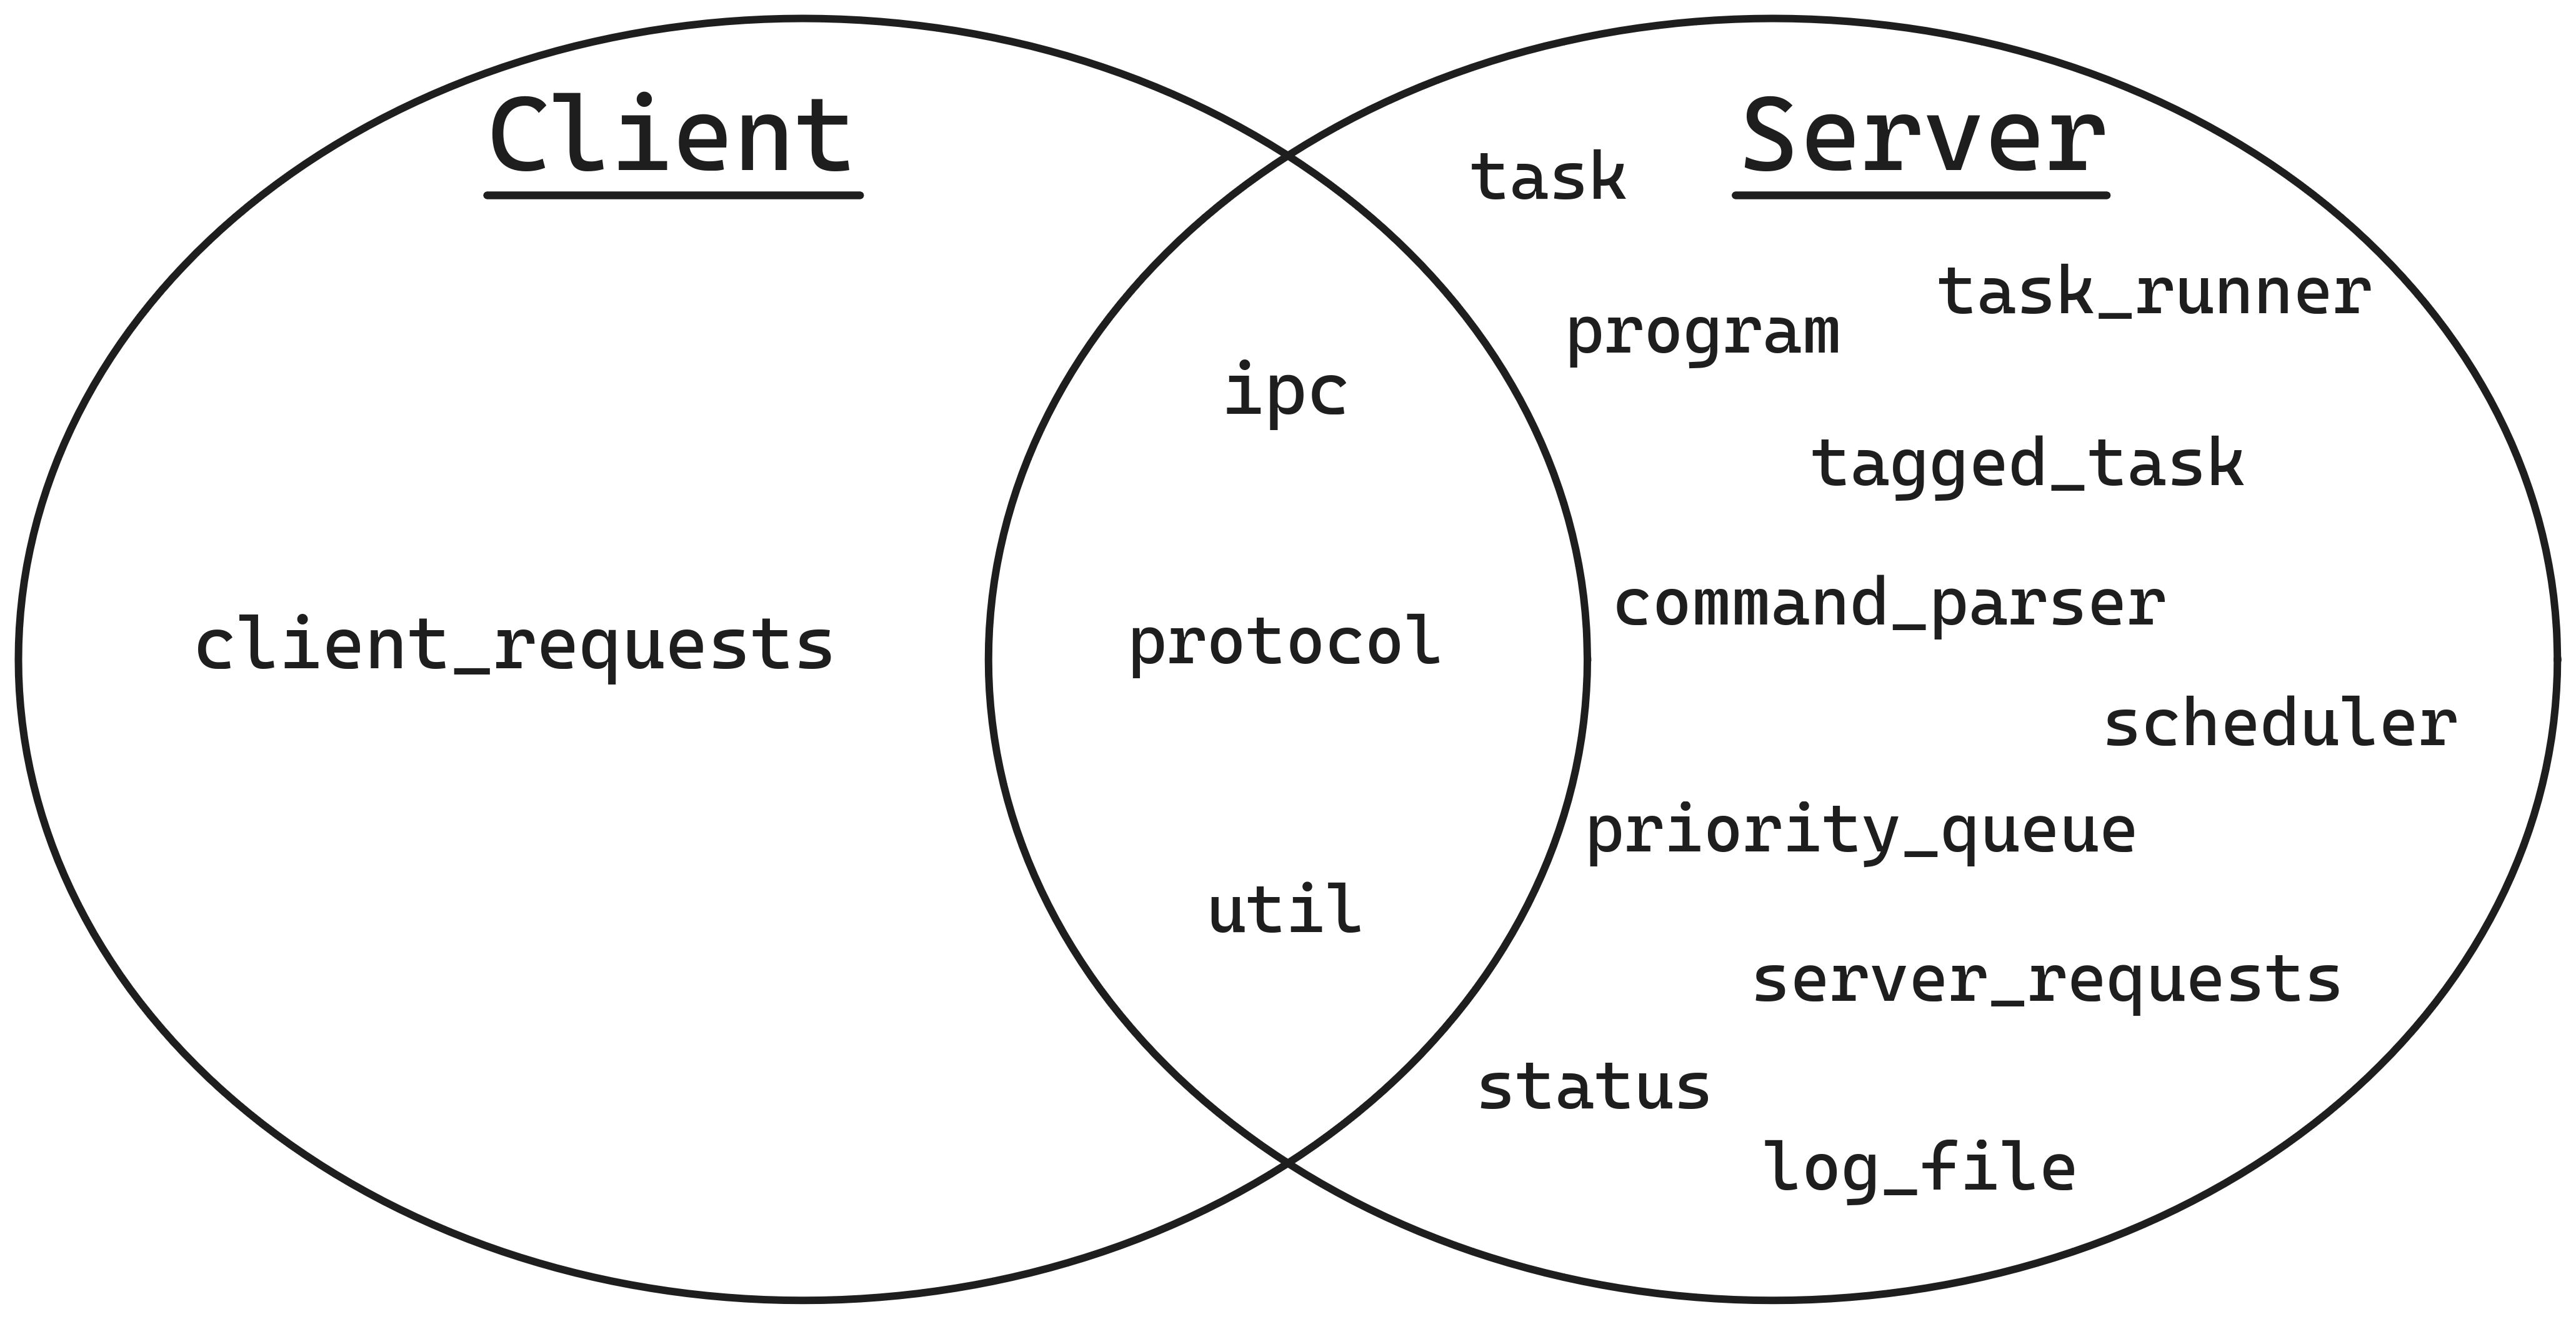
\includegraphics[width=0.6\textwidth]{report_figures/modules_venn_diagram.png}
    \caption{Módulos presentes no cliente e no servidor.}
\end{figure}

Alguns módulos são partilhados pelo cliente e pelo servidor: \texttt{util} fornece utilidades de
escrita para \texttt{stdout} e \texttt{stderr} utilizando a \emph{system call} \texttt{write};
\texttt{ipc} é responsável pela comunicação interprocesso a um nível mais básico (abertura de
conexões e separação de mensagens) utilizando \emph{pipes} com nome, enquanto que em
\texttt{protocol} estão definidas as estruturas das mensagens serializadas, transmitidas entre o
cliente e o servidor, e vice-versa.

O único módulo presente apenas no cliente é \texttt{client\_requests}, que é responsável por enviar
mensagens ao servidor e receber as suas respostas. No servidor, o módulo \texttt{server\_requests}
tem o papel dual: espera por pedidos do cliente para lhes responder. Este módulo é também
responsável por coordenar, conforme as mensagens que são recebidas, as escritas para o ficheiro de
\emph{logs}, feitas pelo módulo \texttt{log\_file}.

Há várias estruturas de dados no servidor. \texttt{program} é um \emph{array} de argumentos
terminado em \texttt{NULL}, facilmente providenciado a uma \emph{system call} na família
\texttt{exec}. Vários programas formam uma \emph{pipeline} em \texttt{task}, que alternativamente
pode ser constituída por um procedimento de C (é possível escalonar tarefas que não programas
independentes). Há mais informação necessária para a gestão de tarefas do que uma lista de
programas, como identificadores e tempos em filas de espera. Uma \texttt{tagged\_task} é formada por
uma \texttt{task} e por esta informação. Continuando-se a cadeia de composição, tem-se a estrutura
\texttt{priority\_queue}, um \emph{minheap} de tarefas, onde definir uma política de escalonamento
se torna tão simples como definir uma função de comparação entre tarefas.

Vários outros módulos são responsáveis pela funcionalidade do servidor. Apesar de uma \texttt{task}
poder ser criada manualmente, programa a programa, a funcionalidade de interpretação de uma
\emph{string} de linha de comandos é providenciada pelo módulo \texttt{command\_parser}.
\texttt{scheduler} é responsável por saber que tarefas estão em execução e em fila de espera,
criando novos processos para a execução de novas tarefas desde que tenha disponibilidade para tal.
Há dois programas que são executados, \texttt{status}, responsável por enviar ao cliente informação
sobre o servidor sem o bloquear, e \texttt{task\_runner}, responsável pela execução de tarefas
como \emph{pipelines}, informando o processo pai do orquestrador quando estas terminam.

A arquitetura modular utilizada foi essencial para o \emph{software} desenvolvido. Não só garante
código de melhor qualidade, como permite evitar erros (como erros de memória e invariantes violadas)
que ocorrem devido à quebra do encapsulamento. A manutenção do código também se tornou mais simples.
Por exemplo, foi necessária, devido a um \emph{bug} que não se conseguiu resolver, a mudança
completa do protocolo definido em \texttt{ipc.c}. Foi possível reescrever este ficheiro mantendo a
interface das funções nele definidas, e o servidor manteve-se operacional sem qualquer outra mudança
necessária.

\end{document}
